%!TEX root = ../systemnahe-programmierung.tex

\chapter{Implementierung}\label{implementierung}

\begin{figure}[htbp]
\centering
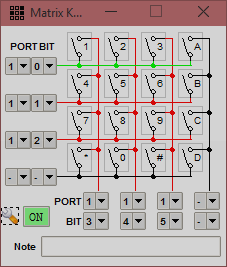
\includegraphics{images/keypad-screenshot}
\caption{Konfiguration des Nummernfeldes}
\end{figure}

Für die Simulation des Nummernfeldes wird das \emph{Matrix Keypad} der \emph{MCU 8051 IDE}
verwendet. Als Erstes muss die Pin-Belegung konfiguriert werden. Im Bild kann man sehen, dass das
Nummerfeld auf Port 1 erreichbar ist. Diese Einstellung kann auch in die IDE import werden (siehe
Anhang).

\begin{lstlisting}
keypad      equ P1              ;Matrix keypad
col1        equ keypad.3        ;Column 1
col2        equ keypad.4        ;Column 2
col3        equ keypad.5        ;Column 3

value       equ 30H             ;Value of pressed button
pressed     bit 00H             ;Was the button just pressed?
secure_mode bit 01h             ;Is the user logiged in?
\end{lstlisting}

Zusätzlich zu den Bits für das Nummernfeld werden auch noch drei Variablen definiert:

\begin{itemize}
\item
  \mintinline{text}{value}: Wert der gedrückten Taste
\item
  \mintinline{text}{pressed}: Ob schon eine Taste gedrückt wurde (wird zurückgesetzt, wenn auf ein neuen
  Tastendruck gewartet wird)
\item
  \mintinline{text}{secure_mode}: In welchem Zustand die Alarmsicherung ist (0 für ausgeschaltet, 1 für
  eingeschaltet)
\end{itemize}

\begin{lstlisting}
get_button:
    clr pressed

    ;Check first row
    mov value,#1                ;Start value is first number on row
    mov keypad, #11111110B      ;Mark first row
    acall check_col1            ;Check all columns 

    ;If button was pressed in row, jump out of function
    jb pressed, found_button    
 
    mov value,#4
    mov keypad, #11111101B
    acall check_col1
 
    jb pressed, found_button
 
    mov value,#7
    mov keypad, #11111011B
    acall check_col1
 
    jb pressed, found_button

    jmp get_button
\end{lstlisting}

Die Zeilen des Nummernfeldes werden nacheinander überprüft. Dabei wird zuerst \mintinline{text}{value} auf
den Wert der ersten Taste aus der Reihe gesetzt. Danach werden alle Reihen außer die ausgewählte auf
\mintinline{text}{1} gesetzt und zur Funktion \mintinline{text}{check_col1} gesprungen, die die Spaltenüberprüfung
für die ausgewählte Reihe startet. Nach jeder Reihe wird überprüft, ob schon eine Taste gedrückt
wird. Ist dies der Fall, dann wird aus der Funktion gesprungen. Wenn alle Reihen überprüft worden
sind und kein Tastendruck erkannt wurde, dann wird die Überprüfung wieder von vorne angefangen.

\begin{lstlisting}
check_col1:
    ;If button wasn't pressed, jump to next colum
    jb col1, check_col2

    ;If button was pressed, wait for end of button press
    jnb col1,$

    ;Set bit that key was pressed
    setb pressed
    ret
\end{lstlisting}

Wenn in der ersten Spalte kein Tastendruck entdeckt worden ist, wird zu \mintinline{text}{check_col2}
gesprungen, die die nächste Spalte überprüft. Sollte die Taste aber gedrückt sein, dass muss erst
auf das Ende des Tastendrucks gewartet werden. Dafür wird einfach zur gleichen Zeile der Überprüfung
gesprungen. Dach wird noch das Bit für \mintinline{text}{pressed} auf \mintinline{text}{1} gesetzt.

\begin{lstlisting}
check_col2:
    jb col2, check_col3
    jnb col2,$
    inc value           ;Increment the start value from row
    setb pressed
    ret
\end{lstlisting}

Die Überprüfung der nächsten Spalten funktioniert fast identisch. Der einzige Unterschied findet bei
einem erfolgreichem Tastendruck statt. Da der Wert der Taste verschiedene Werte hat, muss der Inhalt
von \mintinline{text}{value} noch angepasst werden. Dafür wird einfach um den Unterschied inkrementiert (in
diesem Fall 1).

\begin{lstlisting}
check_pin:
    ;Check first pin (4)
    acall get_button
    mov A, value
    cjne A, #4, check_pin

    ;Check second pin (2)
    acall get_button
    mov A, value
    cjne A, #2, check_pin

    ;Check third pin (6)
    acall get_button
    mov A, value
    cjne A, #6, check_pin

    ;Check fourth pin (8)
    acall get_button
    mov A, value
    cjne A, #8, check_pin

    ;Toggle secure mode of the system
    cpl secure_mode
\end{lstlisting}

Die Hauptfunktion ist \mintinline{text}{check_pin}. Sie ruft viermal die \mintinline{text}{get_button}-Funktion
auf und überprüft, ob der gelieferte Tastendruck dem gewünschtem gleicht. Sollte dies einmal nicht
der Fall sein, dann wird die Suche von vorne angefangen. Aber wurde die Ziffernfolge erfolgreich
eingegeben, dann wird der Alarm-Modus gewechselt. Die Zifferfolge lässt sich sehr leicht ändern,
unter anderem auch in der Länge.